\chapter{Numeri Complessi}\label{numeri-complessi}
L'equazione
\[
x^2 + 1 = 0
\]
non ha soluzioni in $\mathbb{R}$. Dobbiamo quindi ampliare l'insieme $\mathbb{R}$ per fare in modo che le equazioni algebriche di questo tipo ammettano soluzioni.

\section{Il campo dei numeri complessi}
Chiamiamo $\mathbb{C}$ l'insieme formato dalle coppie ordinate di numeri reali appartenenti al prodotto $\mathbb{R} \times \mathbb{R}$. Definiamo su questo insieme due operazioni binarie interne (rispettivamente somma e prodotto):
\begin{itemize}
    \item \textbf{Somma:} $(a, b) + (c, d) = (a+c, b+d)$
    \item \textbf{Prodotto:} $(a, b) \cdot (c, d) = (ac - bd, ad + bc)$
\end{itemize}

La struttura $(\mathbb{C}, +, \cdot)$ soddisfa tutti gli assiomi di campo e prende il nome di \emph{campo complesso}:
\begin{enumerate}
    \item $\forall \alpha, \beta, \gamma \in \mathbb{C}$ valgono le proprietà commutativa, associativa e distributiva.
    
    \item $(0, 0)$ costituisce l'elemento neutro rispetto alla somma (zero), mentre $(1, 0)$ è l'elemento neutro rispetto al prodotto (unità).
    
    \item L'opposto della coppia $(a, b)$ è la coppia $(-a, -b)$. Per ogni $(a, b) \neq (0, 0)$, il reciproco (o inverso) è la coppia:
    \[
        (a, b)^{-1} = \left( \frac{a}{a^2+b^2}, \frac{-b}{a^2+b^2} \right)
    \]
\end{enumerate}

Indichiamo con $R$ il sottoinsieme di $\mathbb{C}$ formato dalle coppie $(a, 0)$, con $a \in \mathbb{R}$.
L'applicazione 
\[
    \phi : R \to \mathbb{R}
\]
definita da $\phi((a, 0)) = a$ è un isomorfismo tra il campo $(R, +, \cdot)$ e il campo $(\mathbb{R}, +, \cdot)$.

$R$ è quindi un sottocampo di $\mathbb{C}$ isomorfo a $\mathbb{R}$. Per convenzione, si identifica $\mathbb{R}$ con questo sottocampo e si scrive $\mathbb{R} \subset \mathbb{C}$.

Consideriamo adesso il numero complesso $(0, 1)$ che viene denotato con il simboli $i$ (unità immaginaria). Notiamo che:
\[
i^2 = (0, 1) \cdot (0, 1) = (-1, 0) = -1
\]
Questa risulta essere proprio una soluzione dell'equazione $x^2 + 1 = 0$.

\section{Forma algebrica}
I numeri complessi possono essere espressi in forma algebrica. Osserviamo ad esempio che:
\[
(0, b) = (b, 0) \cdot (0, 1) = b \cdot i \quad \forall b \in \mathbb{R}
\]

Quindi un qualsiasi numero complesso $(a, b)$ può essere espresso nella forma $a + b \cdot i$:
\[
(a, b) = (a, 0) + (0, b) = (a, 0) + ((b, 0) \cdot (0, 1)) = a + b \cdot i
\]
La forma algebrica è molto comoda perché ci permette di operare sui numeri complessi con le comuni regole del calcolo letterale.

Dato un numero complesso $\alpha = a + bi$, valgono le seguenti definizioni:
\begin{itemize}
    \item $a = \text{Re}(\alpha)$ prende il nome di \emph{parte reale}.
    \item $b = \text{Im}(\alpha)$ prende il nome di \emph{parte immaginaria}.
    \item $\overline{\alpha} = a - bi$ prende il nome di \emph{coniugato} di $\alpha$.
      \ex{
\[
\frac{3 - 2i}{5 + i} \cdot \frac{\overline{z}}{\overline{z}} = \frac{(3-2i)(5-i)}{(5+i)(5-i)} =\frac{(3-2i)(5-i)}{26}
\]
}
      
    
    \item Per ottenere la parte reale di un numero complesso $\alpha$:
    \[
        \text{Re}(\alpha) = \frac{\alpha + \overline{\alpha}}{2}
    \]
    
    \item Per ottenere la parte immaginaria di un numero complesso $\alpha$:
    \[
        \text{Im}(\alpha) = \frac{\alpha - \overline{\alpha}}{2i}
    \]
    
    \item Ne deriva che $\alpha$ è un numero reale se e solo se coincide con il suo coniugato:
    \[
        \alpha = \overline{\alpha} \iff \alpha \in \mathbb{R} \text{ (ovvero, } b = 0 \text{)}
    \]
  \end{itemize}
  
\subsection{Operazioni}
Dati due numeri complessi $z_1 = x_1 + y_1i$ e $z_2 = x_2 + y_2i$:
\begin{itemize}
  \item Somma:
  \[
    z_1 + z_2 = (x_1 + x_2) + (y_1 + y_2)i
  \]

  \item Prodotto:
  \[
    z_1 \cdot z_2 = (x_1x_2 - y_1y_2) + (x_1y_2 + x_2y_1)i
  \]

  \item Per effettuare la divisione di due numeri complessi dobbiamo effettuare un processo simile alla razionalizzazione delle radici.  
  Moltiplichiamo numeratore e denominatore per il \emph{complesso coniugato} del denominatore:
  \[
    \frac{z_1}{z_2} = \frac{z_1}{z_2} \cdot \frac{\overline{z_2}}{\overline{z_2}} = 
    \frac{z_1 \, \overline{z_2}}{|z_2|^2}
  \]
  dove il coniugato di $z_2 = x_2 + y_2i$ è $\overline{z_2} = x_2 - y_2i$, e $|z_2|^2 = x_2^2 + y_2^2$.
\end{itemize}

  \section{Piano complesso}
  Così come $\R$ può essere identificato come l'insieme dei punti di una retta, il campo complesso può essere identificato come l'insieme dei punti di un piano che prende il nome di \emph{piano di Gauss}, dove:
  \begin{itemize}
  \item L'asse delle ordinate prende il nome di asse immaginario
  \item L'asse delle ascisse prende il nome di asse reale
  \end{itemize}
  
    \begin{figure}[H]
    \centering
    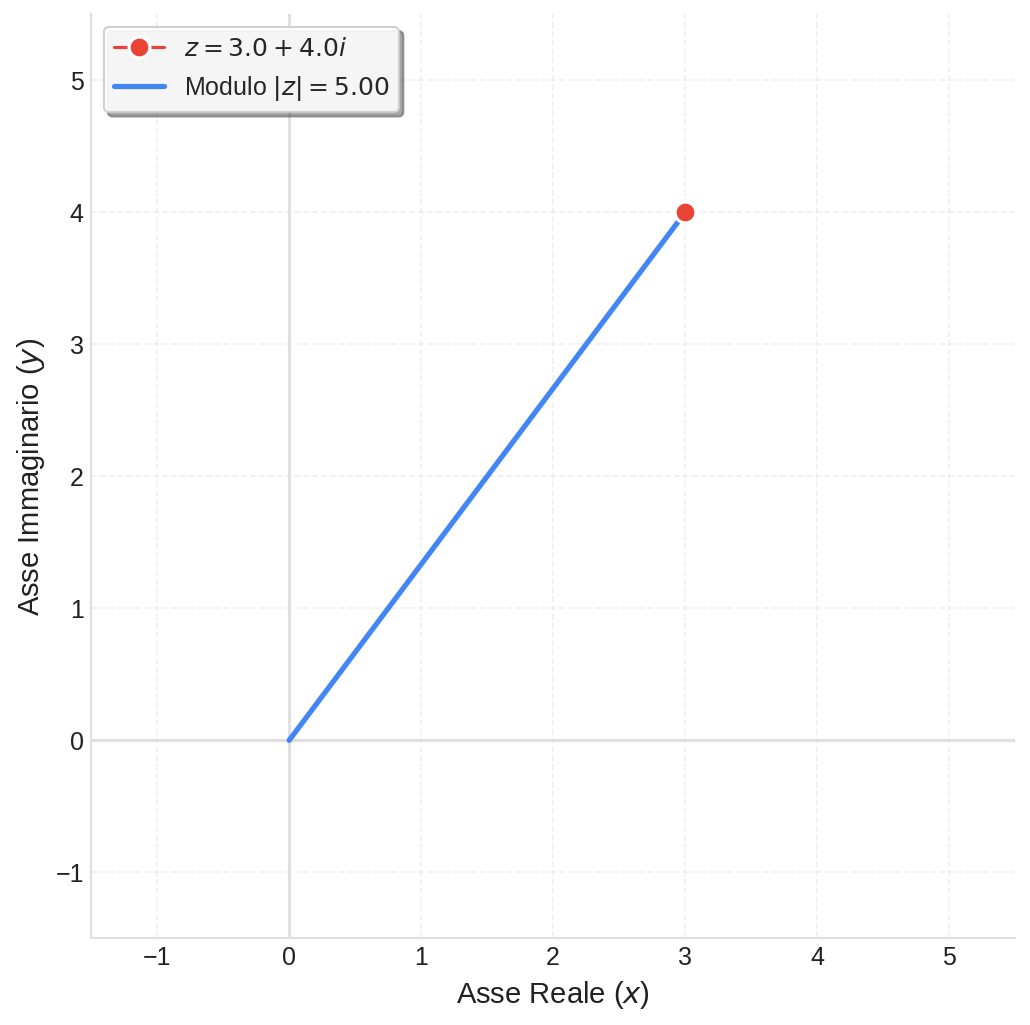
\includegraphics[width=0.75\textwidth]{img/piano_gauss.png}
  \end{figure}

  \subsection{Modulo}
  Geometricamente nel piano di Gauss la lunghezza del segmento che congiunge un punto del piano identificato da un numero complesso $z = x + yi$ con l'origine si indica con $|z|$:
  \[
\sqrt(x^2+y^2) = |z|
\]

\ex{
\[\begin{array}{l}
z_1 = 2i \quad z_2 = 3 - i \\
|z_1 - z_2| = |2i - 3 + i| = |-3 + 3i| = 3\sqrt{2}
\end{array}\]
}
\section{Forma trigonometrica}
\defn{Forma trigonometrica}{
\[
\begin{array}{l}
x = \rho \cos \theta , \quad y = \rho \sin \theta \\
\tan \theta = \frac{y}{x} \\
\text{ALLORA} \quad z = \rho[\cos\theta+i\sin\theta]
\end{array}
\]
}

La forma trigonometrica (o in coordinate polari) di un numero complesso ci permette di identificare un qualsiasi $z \in \mathbb{C}$ mediante due valori detti \emph{modulo} e \emph{argomento}.

Abbiamo già visto che il modulo di un numero complesso rappresenta la distanza del punto $P$ identificato dalla coppia $(x, y)$ dall'origine.

L'\emph{argomento} di un numero complesso (necessariamente diverso da 0) è il numero reale $\theta$ che esprime la misura, in radianti, dell'angolo che il semiasse positivo delle ascisse forma con la semiretta $OP$. Si indica con:
\[arg(z) = \{\theta + 2k\pi, \; k \in \mathbb{Z}\}\]

\defn{Argomento principale}{
\(\theta\) non è univocamente determinato.
Si chiama \textbf{argomento principale} \(\theta \in ]-\pi, \pi]\), che
diventa univocamente determinato.\\
Abbiamo così un cambio in \textbf{coordinate polari}, \(\rho\) e
\(\theta\).
}

\begin{figure}[H]
  \centering
  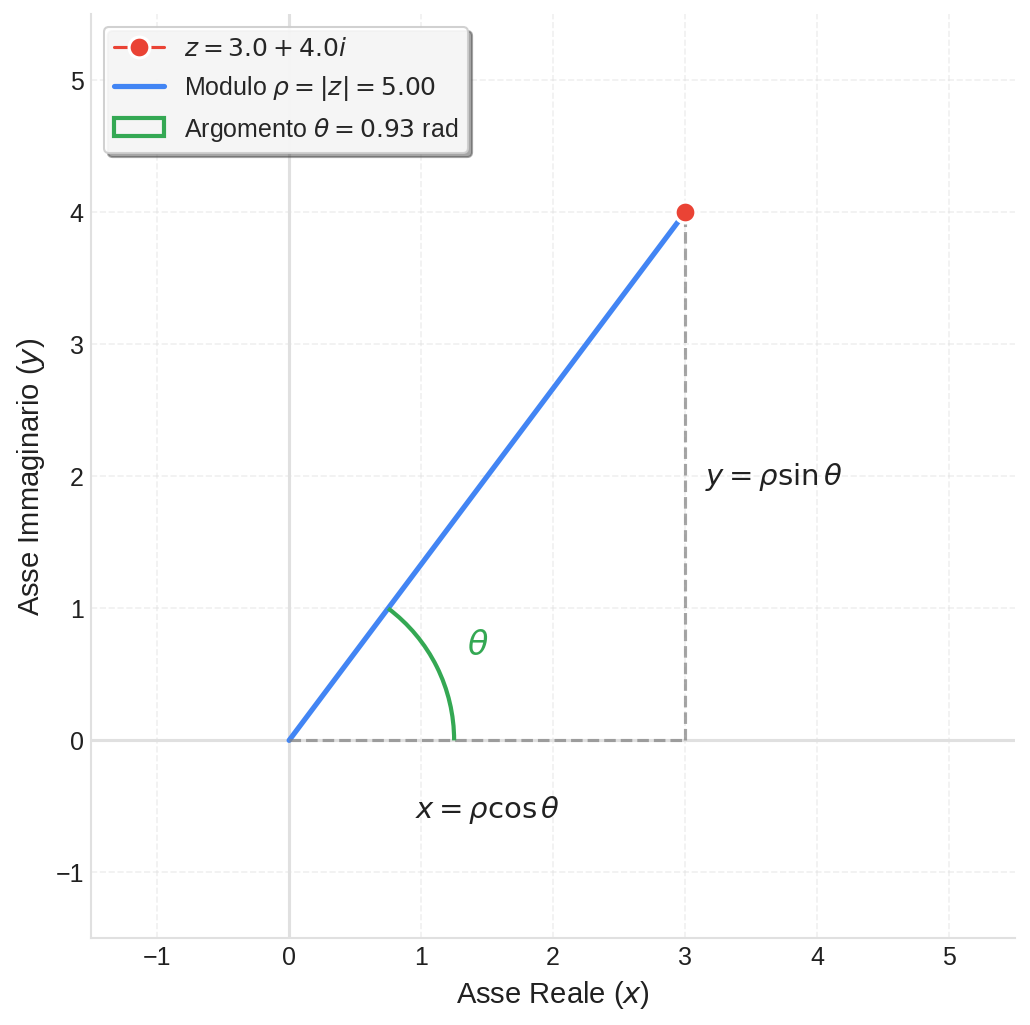
\includegraphics[width=0.75\textwidth]{img/piano_gauss_trigonometrico.png}
\end{figure}

Come si può notare dalla figura, siamo in grado di individuare qualsiasi numero complesso $z = x + yi$ conoscendo la misura del segmento $\overline{OP}$ (modulo di $z$, che indicheremo con $\rho$) e l'ampiezza dell'angolo $\theta$ che $\overline{OP}$ forma con l'asse delle ascisse (argomento di $z$).

Dai teoremi sui triangoli rettangoli risulta che:
\begin{itemize}
  \item $x = \rho \cdot \cos(\theta)$
  \item $y = \rho \cdot \sin(\theta)$
\end{itemize}

Se $\rho$ e $\theta$ sono rispettivamente il modulo e l'argomento, otteniamo la seguente forma trigonometrica del numero complesso:
\[
z = \rho \cos(\theta) + \rho \sin(\theta)i = \rho (\cos(\theta) + i\sin(\theta))
\]
Per convertire un numero complesso dalla forma algebrica alla forma trigonometrica basta ricordare che:
\begin{itemize}
  \item $\rho = \sqrt{x^2 + y^2}$
  \item 
  L'argomento $\theta$ si calcola nel seguente modo:
  \[
  \theta =
  \begin{cases}
    \arctan\!\left(\dfrac{y}{x}\right), & \text{se } x > 0 \\
    \arctan\!\left(\dfrac{y}{x}\right) + \pi, & \text{se } x < 0 \\
    \dfrac{\pi}{2}, & \text{se } x = 0 \text{ e } y > 0 \\
    \dfrac{3\pi}{2}, & \text{se } x = 0 \text{ e } y < 0
  \end{cases}
  \]
\end{itemize}


\section{Potenze}
Rappresentare i numeri complessi in forma trigonometrica risulta particolarmente utile quando dobbiamo calcolare potenze o prodotti tra numeri complessi.

Per comprendere come avviene l’elevamento a potenza, consideriamo innanzitutto il prodotto tra due numeri complessi espressi in forma trigonometrica.  
Siano
\[
z_1 = \rho_1(\cos(\theta_1) + i\sin(\theta_1)) \quad \text{e} \quad 
z_2 = \rho_2(\cos(\theta_2) + i\sin(\theta_2)).
\]
Allora:
\[
z_1 \cdot z_2 = \rho_1 \rho_2 [\cos(\theta_1)\cos(\theta_2) - \sin(\theta_1)\sin(\theta_2) + i(\sin(\theta_1)\cos(\theta_2) + \cos(\theta_1)\sin(\theta_2))].
\]

Applicando le formule goniometriche di somma per seno e coseno, otteniamo:
\[
z_1 \cdot z_2 = \rho_1 \rho_2 [\cos(\theta_1 + \theta_2) + i\sin(\theta_1 + \theta_2)].
\]

\section{Formula di De Moivre}\label{formula-di-de-moivre}
\prop{
Per ogni numero complesso $z = \rho(\cos(\theta) + i\sin(\theta))$ e per ogni intero $n$, vale la seguente relazione:
\[
z^n = \rho^n [\cos(n\theta) + i\sin(n\theta)]
\]
che prende il nome di \emph{formula di De Moivre}.
}

\ex{
\[
\begin{aligned}
&(-1+i)^5 \quad (-1+i)=z\\
&\rho = \sqrt{2}\\
&Arg(z) = \frac{3}{4}\pi\\
&z=\sqrt{2}[\cos{\frac{3}{4}\pi}+i\sin{\frac{3}{4}\pi}]\\
&z^5=\sqrt{2}[\cos{\frac{15}{4}\pi}+i\sin{\frac{15}{4}\pi}]= 4\sqrt{2}[\frac{\sqrt{2}}{2}-\frac{\sqrt{2}}{2}i]=\\
&= 4(1-i)
\end{aligned}
\]
}

\section{Forma esponenziale}
\defn{Formula di Eulero}{
\[e^{i\theta} = \cos \theta + i \sin \theta\]

Non conosciamo ancora il significato di questa funzione, lo vedremo in
\emph{Metodi Matematici per la Fisica (Analisi 3)}.
}

Un numero complesso espresso in forma trigonomerica è rappresentabile anche in forma esponenziale facendo uso della formula di Eulero:
\[
z = \rho(\cos(\theta) + i\sin(\theta)) = \rho e^{i\theta}
\]

Il coniguato si indica con $\rho e^{-i\theta}$. Inoltre $e^{-1\pi} + 1 = 0$.
\section{Radice n-esima}

\defn{Definizione}{
Sia \(n \in \mathbb{N}\) e \(z \in \mathbb{C}\). Si chiama
\textbf{radice n-esima di \(z\)} ogni numero complesso \(w\) tale che:
\[
\boxed{w^n = z}
\]

Scriviamo \[
z = \rho (\cos \theta + i \sin \theta),
\] e cerchiamo \(w\) tale che \[
w^n = r (\cos \phi + i \sin \phi)
\]

Applicando la \textbf{formula di de Moivre}, le radici si possono
scrivere come: \[
w_k = r(\cos \phi_k + i \sin \phi_k), \quad k = 0,1,\dots,n-1
\] dove \(\phi_k\) è definito dal sistema: \[
w^n=z \iff 
\left\{
\begin{array}{l}
r = \sqrt[n]{\rho} \\
\phi_k = \frac{\theta + 2 k \pi}{n}, \quad k = [0,1,2,\dots,n-1]
\end{array}
\right.
\]
}

\ex{
\(z^4 = 1 \Rightarrow z = \sqrt[4]{1}\)\\
Dobbiamo calcolare le \textbf{radici quarte di 1}:\\
\(1 = 1 \cdot e^{i0}\) con \(\rho = 1\) e \(\theta = 0\).
\[
\begin{array}{l}
|w_k| = \sqrt[4]{1} = 1 \\[4pt]
\phi_k = \frac{\theta + 2k\pi}{4} = \frac{k\pi}{2}, \quad k = 0,1,2,3
\end{array}
\]

\begin{center}
\begin{tabular}{c | c | l}
\(k\) & \(\phi_k\) (angolo) & \(w_k\) (radice) \\
\hline
0 & \(0\) & \(w_0 = \cos 0 + i\sin 0 = 1\) \\
1 & \(\frac{\pi}{2}\) & \(w_1 = \cos \frac{\pi}{2} + i\sin \frac{\pi}{2} = i\) \\
2 & \(\pi\) & \(w_2 = \cos \pi + i\sin \pi = -1\) \\
3 & \(\frac{3\pi}{2}\) & \(w_3 = \cos \frac{3\pi}{2} + i\sin \frac{3\pi}{2} = -i\)
\end{tabular}
\end{center}

Le radici, quando le troviamo, risultano tutte \textbf{sulla
circonferenza}.
}	
